A Tabela \ref{tab:tempos_merge} apresenta os tempos de execução, em segundos, obtidos para o Merge Sort nos seis tamanhos de instância exigidos pelo trabalho, para cada um dos três tipos de entrada testados.

\begin{table}[htbp]
    \centering
    \begin{tabular}{|l|r|r|r|r|r|r|}
        \hline
         & 10 & 100 & 1.000 & 10.000 & 100.000 & 1.000.000 \\
        \hline
        Crescente & 0,000002 & 0,000002 & 0,000015 & 0,000194 & 0,002070 & 0,021293 \\
        \hline
        Decrescente & 0,000002 & 0,000002 & 0,000014 & 0,000175 & 0,001809 & 0,020753 \\
        \hline
        Random & 0,000002 & 0,000009 & 0,000058 & 0,000551 & 0,006542 & 0,077718 \\
        \hline
    \end{tabular}
    \caption{Tempo de execução (em segundos) do Merge Sort por tamanho e tipo de instância}
    \label{tab:tempos_merge}
\end{table}


O Gráfico \ref{fig:grafico_merge} apresenta esses mesmos dados em escala linear. Os tempos são todos muito pequenos: mesmo para 1.000.000 de elementos o Merge Sort levou menos de 0,08 segundo nas três situações, uma escala milhares de vezes menor que a dos gráficos dos três primeiros algoritmos. As curvas das entradas crescente e decrescente praticamente se sobrepõem, como previsto na análise de complexidade, e ficam abaixo da curva da entrada randômica.

\begin{figure}[htbp]
    \centering
    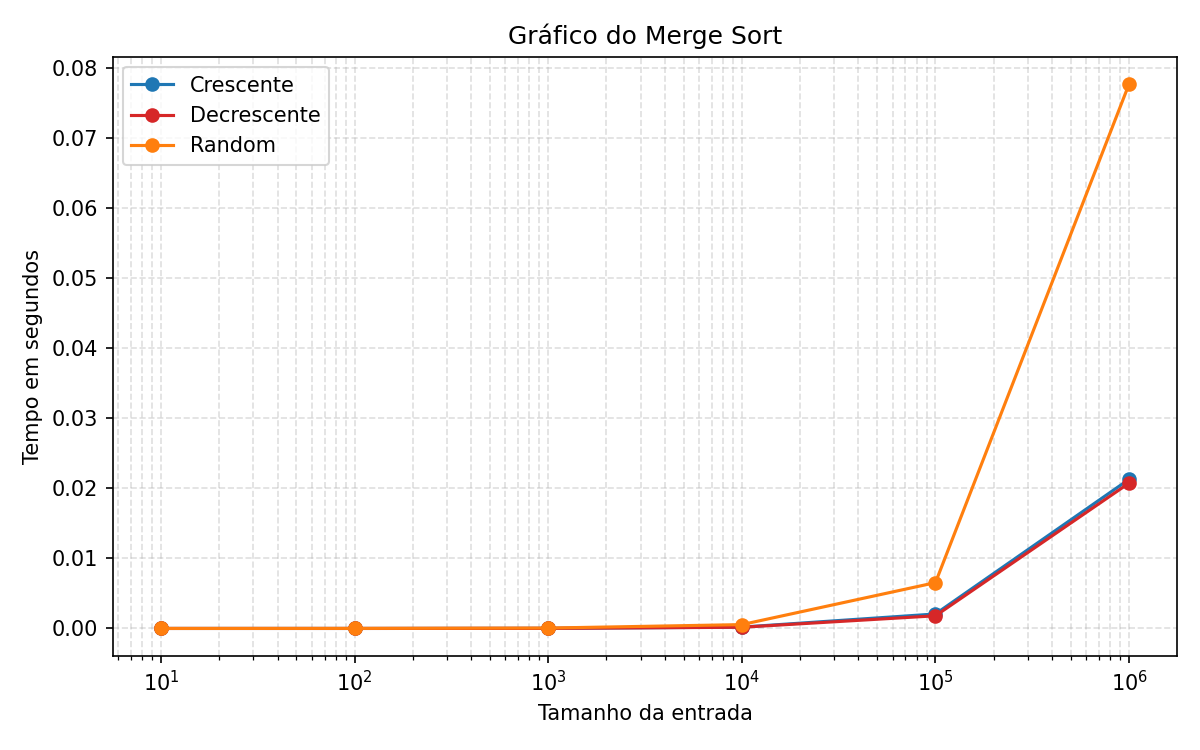
\includegraphics[width=14cm]{Imagens/Merge Sort/grafico.png}
    \caption{Gráfico de tempo por tamanho do algoritmo Merge Sort (escala linear)}
    \label{fig:grafico_merge}
\end{figure}

O Gráfico \ref{fig:grafico_merge_log} apresenta os mesmos dados em escala logarítmica nos dois eixos. Nessa escala, um crescimento quadrático aparece como reta de inclinação 2, e um crescimento da ordem de $n \log n$ como reta de inclinação ligeiramente superior a 1: as três curvas do Merge Sort são aproximadamente paralelas entre si e muito menos inclinadas que as dos algoritmos quadráticos. Quantitativamente, ao aumentar o tamanho da entrada de 100.000 para 1.000.000 de elementos (10 vezes), o tempo foi multiplicado por 10,3 (crescente), 11,5 (decrescente) e 11,9 (randômica), valores próximos de 12,0, que é o fator esperado para $n \log n$ nesse intervalo, e muito distantes de 100, que seria o fator esperado em um crescimento quadrático.

\begin{figure}[htbp]
    \centering
    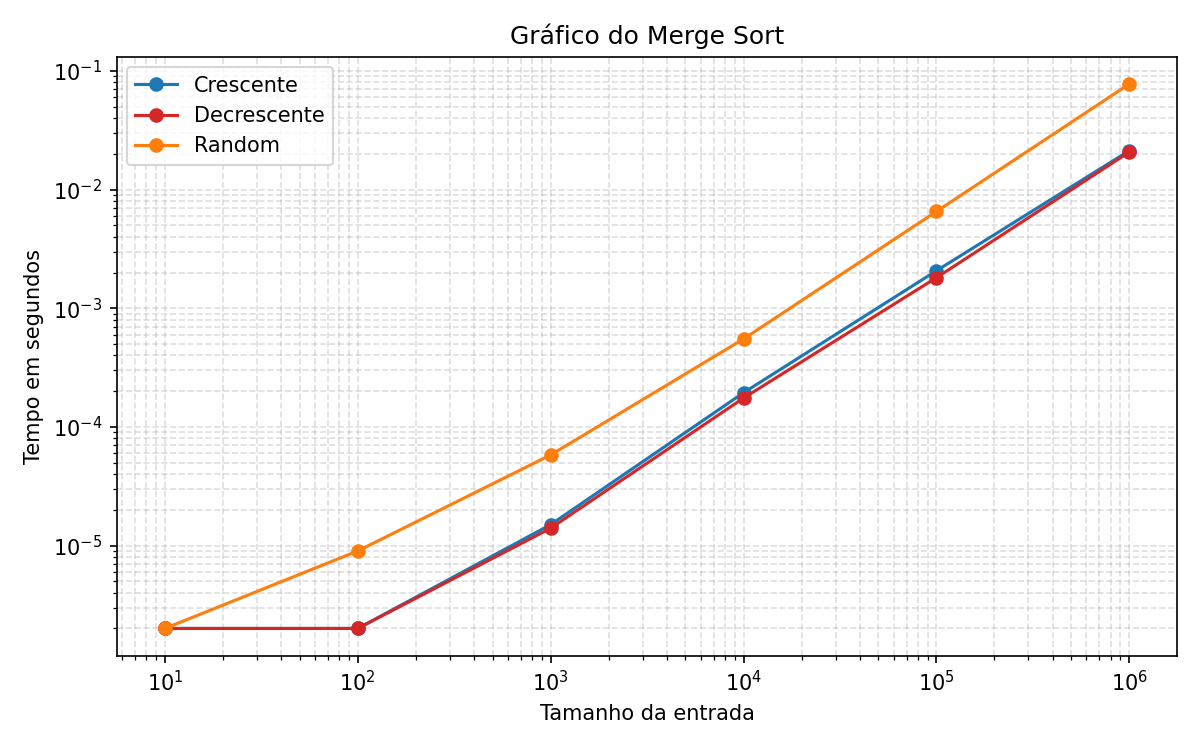
\includegraphics[width=14cm]{Imagens/Merge Sort/grafico_log.png}
    \caption{Gráfico de tempo por tamanho do algoritmo Merge Sort (escala logarítmica)}
    \label{fig:grafico_merge_log}
\end{figure}

A entrada randômica foi a mais lenta: para 1.000.000 de elementos, 0,077718 s, cerca de 3,7 vezes o tempo das entradas ordenadas. Isso não altera a ordem de complexidade, mas merece uma explicação: a entrada randômica exige quase o dobro de comparações (18,7 milhões contra cerca de 10 milhões) e o mesmo número de cópias (39,9 milhões), o que por si só não explicaria uma diferença de 3,7 vezes. Uma explicação plausível, não verificada neste trabalho, é a previsão de desvios do processador: nas entradas ordenadas o resultado de \texttt{vetor[i] <= vetor[j]} segue um padrão regular, que o processador aprende a prever, enquanto na entrada randômica ele é imprevisível e causa perdas de desempenho que a contagem de operações não captura.
